\chapter{Descrizione dello Scenario Specifico dell'Idea Progettuale}

\section{Lo scenario specifico}

L'analisi del contesto svolta nel capitolo precedente ha delineato un quadro ampio, comprensivo di tutti i soggetti che, a vario titolo, gravitano attorno al mondo dell'automotive tuning. Al fine di definire un'idea progettuale concreta e realizzabile, è necessario restringere tale quadro a uno \textbf{scenario specifico}, individuando gli attori che interagiscono direttamente con la piattaforma e i ruoli da essi assunti all'interno del sistema.

Il settore della personalizzazione dei veicoli ha assunto negli ultimi anni una rilevanza economica crescente, accompagnata però da una persistente opacità informativa. Le modifiche apportate a un veicolo --- interventi sulla meccanica, sull'assetto, sull'impianto frenante o sull'estetica --- vengono documentate attraverso fatture, dichiarazioni di conformità e annotazioni sul libretto di circolazione, ossia strumenti eterogenei, facilmente smarribili e non verificabili in modo indipendente. Al momento della rivendita, l'acquirente non dispone di alcuno strumento affidabile per accertare quali lavorazioni siano state realmente eseguite, da chi, con quali componenti e nel rispetto di quali requisiti di omologazione.

Questa asimmetria informativa produce conseguenze concrete su tutta la filiera: l'Azienda di Tuning non riesce a valorizzare la qualità del proprio operato né a tutelarsi da contestazioni infondate; la Concessionaria assume un rischio legale nel commercializzare un veicolo modificato di cui non può dimostrare la piena conformità; il Centro di Certificazione deve ricostruire manualmente la storia degli interventi prima di poter procedere al collaudo; il Cliente Privato, infine, subisce una perdita di valore del proprio veicolo al momento della rivendita, non potendo dimostrare la regolarità e la qualità delle personalizzazioni.

L'idea progettuale, denominata \textit{Tuning Ledger}, risponde a queste criticità attraverso il \textbf{Digital Modified Vehicle Passport} (DMVP): un passaporto digitale immutabile, associato univocamente al numero di telaio del veicolo, che accompagna il mezzo lungo l'intero ciclo di vita registrando in modo verificabile ogni modifica e ogni certificazione. La piattaforma adotta un'architettura ibrida, nella quale i dati descrittivi e la documentazione voluminosa risiedono in un database \textit{off-chain}, mentre sulla blockchain viene ancorata la sola impronta crittografica (\textit{hash}) che ne garantisce l'integrità.

La piattaforma è concepita per offrire servizi personalizzati ai seguenti stakeholder:

\begin{enumerate}
    \item \textbf{Intermediario}, in quanto soggetto che sviluppa e gestisce la piattaforma, interessato a fornire un'infrastruttura di tracciabilità affidabile agli attori della filiera e a verticalizzare la soluzione sulle loro specifiche esigenze.
    \item \textbf{Concessionaria}, in quanto interessata a differenziare la propria offerta commerciale con un servizio premium e a ridurre il rischio legale connesso alla vendita di veicoli modificati, potendo dimostrare la conformità di ogni intervento.
    \item \textbf{Azienda di Tuning}, in quanto interessata ad attestare digitalmente la qualità del proprio lavoro, tutelandosi da contestazioni infondate attraverso la registrazione immutabile delle lavorazioni eseguite e dei componenti installati.
    \item \textbf{Centro di Certificazione}, in quanto interessato a disporre di dati verificabili e già strutturati per l'esecuzione del collaudo, riducendo i tempi di verifica, e a registrare i certificati emessi in modo che siano controllabili da terzi.
    \item \textbf{Cliente Privato}, in quanto interessato a verificare l'autenticità delle modifiche apportate al proprio veicolo e a disporre di uno storico certificato e trasferibile, che ne accresce il valore al momento della rivendita.
\end{enumerate}

Restano invece esclusi dallo scenario specifico, pur essendo stati individuati nell'analisi del contesto, i soggetti che non interagiscono direttamente con la piattaforma ma con i quali essa si interfaccia in qualità di \textbf{partner}: la Motorizzazione Civile, competente per l'omologazione delle modifiche; la Casa Automobilistica, che fornisce i dati ufficiali del veicolo base; i Fornitori di componenti, che ne attestano la provenienza; e le Aziende di spedizione, coinvolte nella logistica di consegna.

\section{Contesto tecnologico: tecnologie e soluzioni già disponibili}

\subsection{Tecnologie rilevanti}

Il contesto tecnologico dell'idea progettuale è caratterizzato dalla necessità di gestire informazioni critiche relative al ciclo di vita dei veicoli, in particolare per quanto riguarda modifiche, manutenzioni e interventi certificati. In tale scenario risulta fondamentale adottare soluzioni in grado di garantire \textbf{integrità, tracciabilità e verificabilità} dei dati, riducendo le asimmetrie informative tra i diversi attori coinvolti.

In questo ambito la \textbf{blockchain} si configura come una tecnologia rilevante per lo sviluppo di sistemi informativi distribuiti orientati alla collaborazione tra organizzazioni. Essa può essere definita come un \textbf{registro distribuito} (\textit{Distributed Ledger Technology}, DLT) in cui le informazioni vengono registrate in modo immutabile e condiviso tra più nodi della rete, senza la necessità di un'autorità centrale di controllo. Le principali caratteristiche di interesse per il progetto sono:

\begin{itemize}
    \item \textbf{immutabilità dei dati}, che garantisce la non alterabilità delle informazioni storiche;
    \item \textbf{tracciabilità}, che consente di ricostruire in modo affidabile l'evoluzione delle modifiche apportate a un veicolo;
    \item \textbf{sicurezza}, ottenuta tramite meccanismi crittografici;
    \item \textbf{condivisione controllata}, che permette a più attori di accedere a un'unica fonte informativa affidabile.
\end{itemize}

Un elemento centrale della blockchain è il \textbf{meccanismo di consenso}, attraverso il quale i partecipanti alla rete concordano sulla validità delle informazioni da registrare. Tale meccanismo consente di garantire l'affidabilità del sistema anche in contesti caratterizzati da interessi differenti tra gli stakeholder, come è appunto il caso della filiera del tuning.

Dal punto di vista architetturale è possibile distinguere blockchain \textbf{pubbliche}, aperte e completamente decentralizzate; blockchain \textbf{private}, controllate da un singolo soggetto; e blockchain \textbf{permissioned}, in cui l'accesso è riservato a partecipanti autorizzati. Nel contesto automotive queste ultime risultano particolarmente rilevanti, poiché permettono di bilanciare decentralizzazione e controllo, consentendo la definizione di ruoli e responsabilità per soggetti quali officine, concessionarie ed enti certificatori.

Un ulteriore aspetto tecnologico di rilievo è rappresentato dagli \textbf{smart contract}, programmi eseguiti automaticamente sulla blockchain al verificarsi di determinate condizioni. Essi consentono di automatizzare i processi di validazione e certificazione, riducendo l'intervento manuale e aumentando l'affidabilità delle operazioni. L'integrazione con \textbf{oracoli} permette inoltre di collegare la blockchain a fonti informative esterne, quali gli enti di omologazione.

Nonostante i vantaggi, l'adozione della blockchain introduce alcune criticità, tra cui una maggiore \textbf{complessità architetturale}, la necessità di \textbf{competenze specialistiche} e potenziali \textbf{limiti di scalabilità} in scenari ad alto volume di transazioni. Alla luce di tali considerazioni, la blockchain emerge come tecnologia adeguata all'idea progettuale a condizione che venga adottata in modo mirato e integrata all'interno di un'architettura più ampia, coerente con i requisiti funzionali e organizzativi del sistema informativo.

\subsection{Soluzioni tecnologiche specifiche esistenti}

L'analisi delle soluzioni tecnologiche specifiche si basa sulla valutazione di piattaforme blockchain già adottate in contesti reali affini all'idea progettuale. L'obiettivo è verificare l'esistenza di tecnologie consolidate in grado di soddisfare i casi d'uso individuati, riducendo i rischi di sviluppo e aumentando l'affidabilità complessiva del sistema. I principali requisiti tecnologici del progetto possono essere sintetizzati nell'immutabilità e tracciabilità delle modifiche, nel coinvolgimento di più attori con ruoli distinti, nella verificabilità delle informazioni da parte di terzi, nell'integrazione con sistemi esterni e nella scalabilità con contenimento dei costi operativi.

Nel panorama delle soluzioni esistenti, piattaforme blockchain \textbf{permissioned} come \textbf{Hyperledger Fabric}~\cite{hyperledger} risultano già adottate in ambito automotive per la gestione di registri distribuiti relativi alla storia dei veicoli. Tali soluzioni consentono di registrare in modo sicuro eventi quali manutenzioni, restauri e trasferimenti di proprietà, garantendo trasparenza e immutabilità delle informazioni tra produttori, officine e assicurazioni. L'impiego di Hyperledger Fabric si è dimostrato efficace anche nella documentazione certificata dei processi di restauro delle auto classiche, promuovendo collaborazione, fiducia e aumento del valore di mercato dei veicoli~\cite{murta2024}.

Accanto alle soluzioni permissioned sono stati proposti anche approcci basati su blockchain pubbliche. Un esempio rilevante è rappresentato da architetture che prevedono la \textbf{tokenizzazione del veicolo} tramite l'emissione di un \textbf{NFT} associato al bene fisico~\cite{nftvehicle}: in tali modelli l'intero ciclo di vita del veicolo viene rappresentato attraverso smart contract gerarchici, che registrano transazioni e modifiche in modo strutturato, riducendo il rischio di frodi e asimmetrie informative. Queste soluzioni, spesso implementate su piattaforme come Ethereum, dimostrano la fattibilità tecnica del modello, pur presentando limiti in termini di costi e scalabilità.

Nel contesto dell'automotive tuning l'adozione di una piattaforma blockchain permissioned risulta particolarmente vantaggiosa. Un sistema come il DMVP consente di registrare modifiche estetiche e funzionali corredate dalle relative certificazioni normative, rendendo tali informazioni accessibili tramite applicazioni dedicate o QR code applicato al veicolo. L'utilizzo di smart contract permette inoltre di validare automaticamente la conformità delle modifiche, riducendo il rischio di irregolarità.

Alla luce di queste considerazioni, la soluzione tecnologica più adeguata consiste nell'adozione di una \textbf{blockchain permissioned} integrata all'interno di una piattaforma proprietaria, secondo un'\textbf{architettura ibrida} in cui la blockchain è utilizzata per la registrazione certificata e verificabile delle informazioni critiche, mentre la piattaforma applicativa gestisce la logica di business, l'interazione con gli utenti e l'integrazione con i sistemi esterni. Tale approccio consente di sfruttare tecnologie già validate in ambito automotive, garantendo al contempo flessibilità, controllo dei costi e copertura completa dei requisiti funzionali del progetto.

\section{Modellazione dello Scenario Specifico in GOREM}

Dall'analisi del contesto è stato definito uno scenario specifico che permette di identificare con precisione gli stakeholder direttamente coinvolti nello sviluppo e nell'uso della piattaforma e i diversi ruoli da essi assunti all'interno del sistema. In particolare:

\begin{enumerate}
    \item \textbf{Intermediario}
    \begin{itemize}
        \item \textit{Amministratore della piattaforma}: garantisce il funzionamento, la configurazione e la sicurezza della rete blockchain permissioned, definendo i canali e le politiche di validazione delle transazioni.
        \item \textit{Gestore delle identità e onboarding}: registra e verifica le identità degli attori business, abilitandoli all'uso della piattaforma ed emettendo le credenziali necessarie a operare sulla rete.
        \item \textit{Assistente all'uso}: fornisce assistenza tecnica e operativa agli utenti della piattaforma, accompagnandoli nella configurazione iniziale e nella risoluzione delle anomalie.
    \end{itemize}
    \item \textbf{Concessionaria}
    \begin{itemize}
        \item \textit{Registrante del veicolo base}: registra i dati identificativi del veicolo originale e la richiesta di tuning, creando il passaporto digitale associato al numero di telaio.
        \item \textit{Responsabile della consegna}: consegna il veicolo omologato al Cliente Privato e registra la consegna sul DMVP.
    \end{itemize}
    \item \textbf{Azienda di Tuning}
    \begin{itemize}
        \item \textit{Esecutore della modifica}: esegue le lavorazioni sul veicolo e ne carica in modo permanente la documentazione tecnica, comprensiva dei seriali dei componenti installati.
    \end{itemize}
    \item \textbf{Centro di Certificazione}
    \begin{itemize}
        \item \textit{Ispettore/Collaudatore}: verifica la conformità tecnica e normativa degli interventi eseguiti sul veicolo.
        \item \textit{Emittente della certificazione}: rilascia il certificato di conformità e lo registra in modo immutabile sulla piattaforma.
    \end{itemize}
    \item \textbf{Cliente Privato}
    \begin{itemize}
        \item \textit{Consultatore dello storico}: consulta in qualsiasi momento lo storico immutabile e completo delle modifiche del veicolo.
        \item \textit{Acquirente/Nuovo proprietario}: accetta il veicolo al termine della consegna e ne riceve la proprietà del passaporto digitale.
    \end{itemize}
\end{enumerate}

Quanto descritto è illustrato nella Figura~\ref{fig:role-diagram}.

\begin{figure}[H]
    \centering
    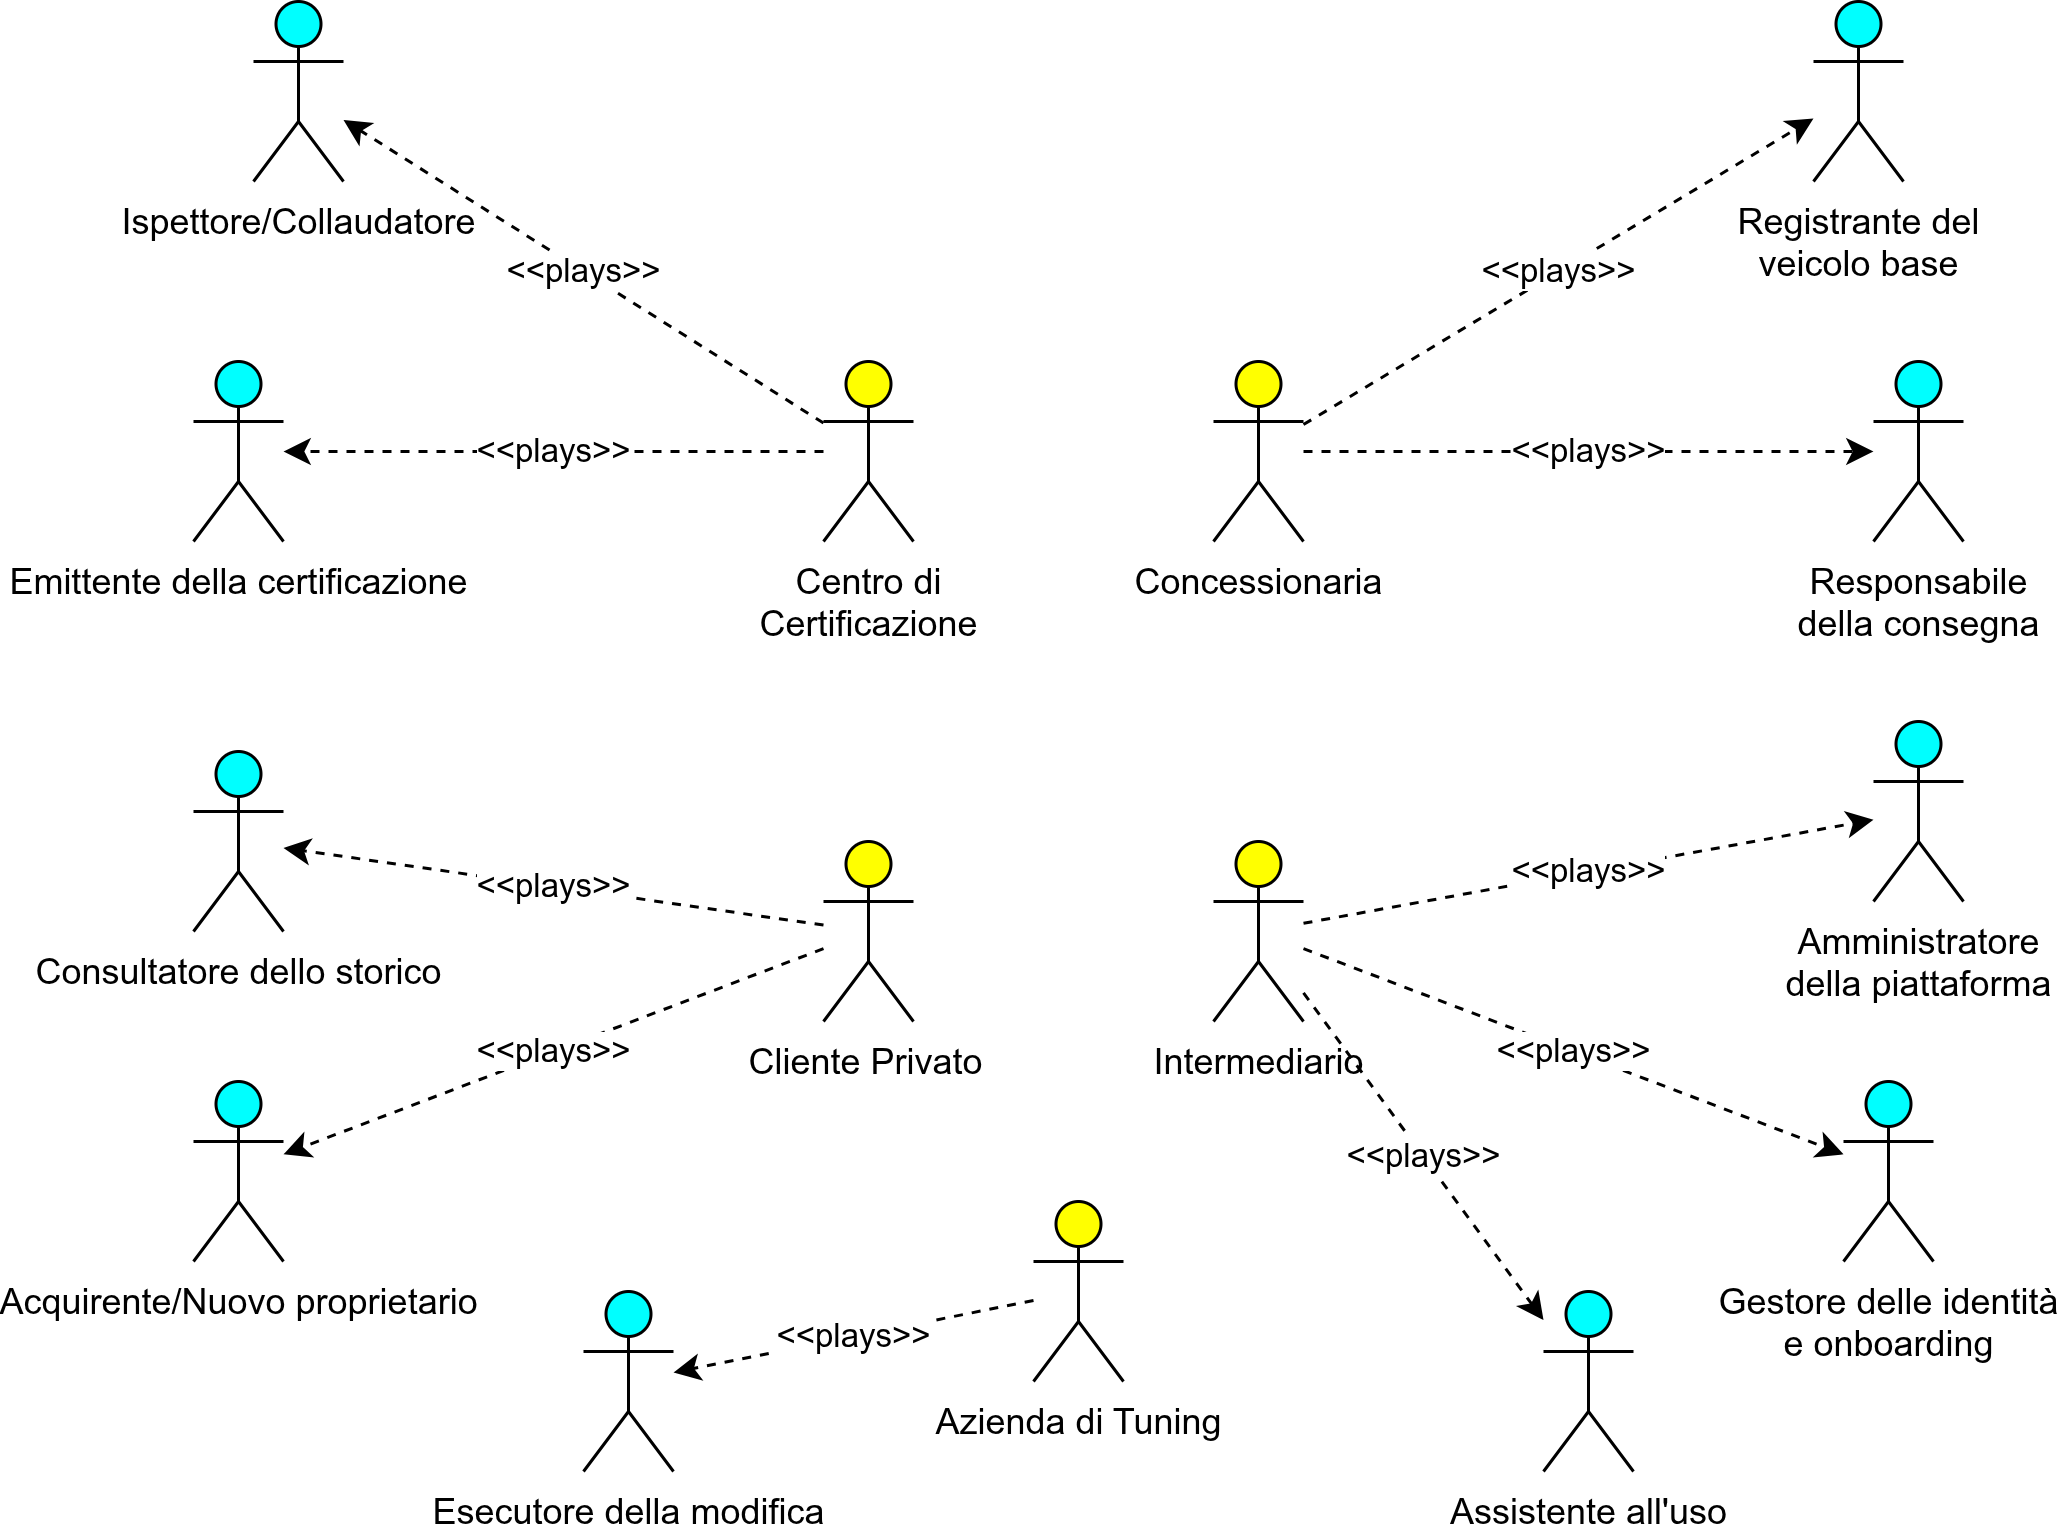
\includegraphics[width=\textwidth]{imgs/scenario/role_diagram.png}
    \caption{Role Diagram}
    \label{fig:role-diagram}
\end{figure}

La Figura~\ref{fig:goal-diagram} presenta i goal specifici associati a ciascun ruolo nello scenario. Coerentemente con l'impostazione adottata, a ogni ruolo corrisponde un unico obiettivo, che ne sintetizza la responsabilità all'interno del sistema.

\begin{figure}[H]
    \centering
    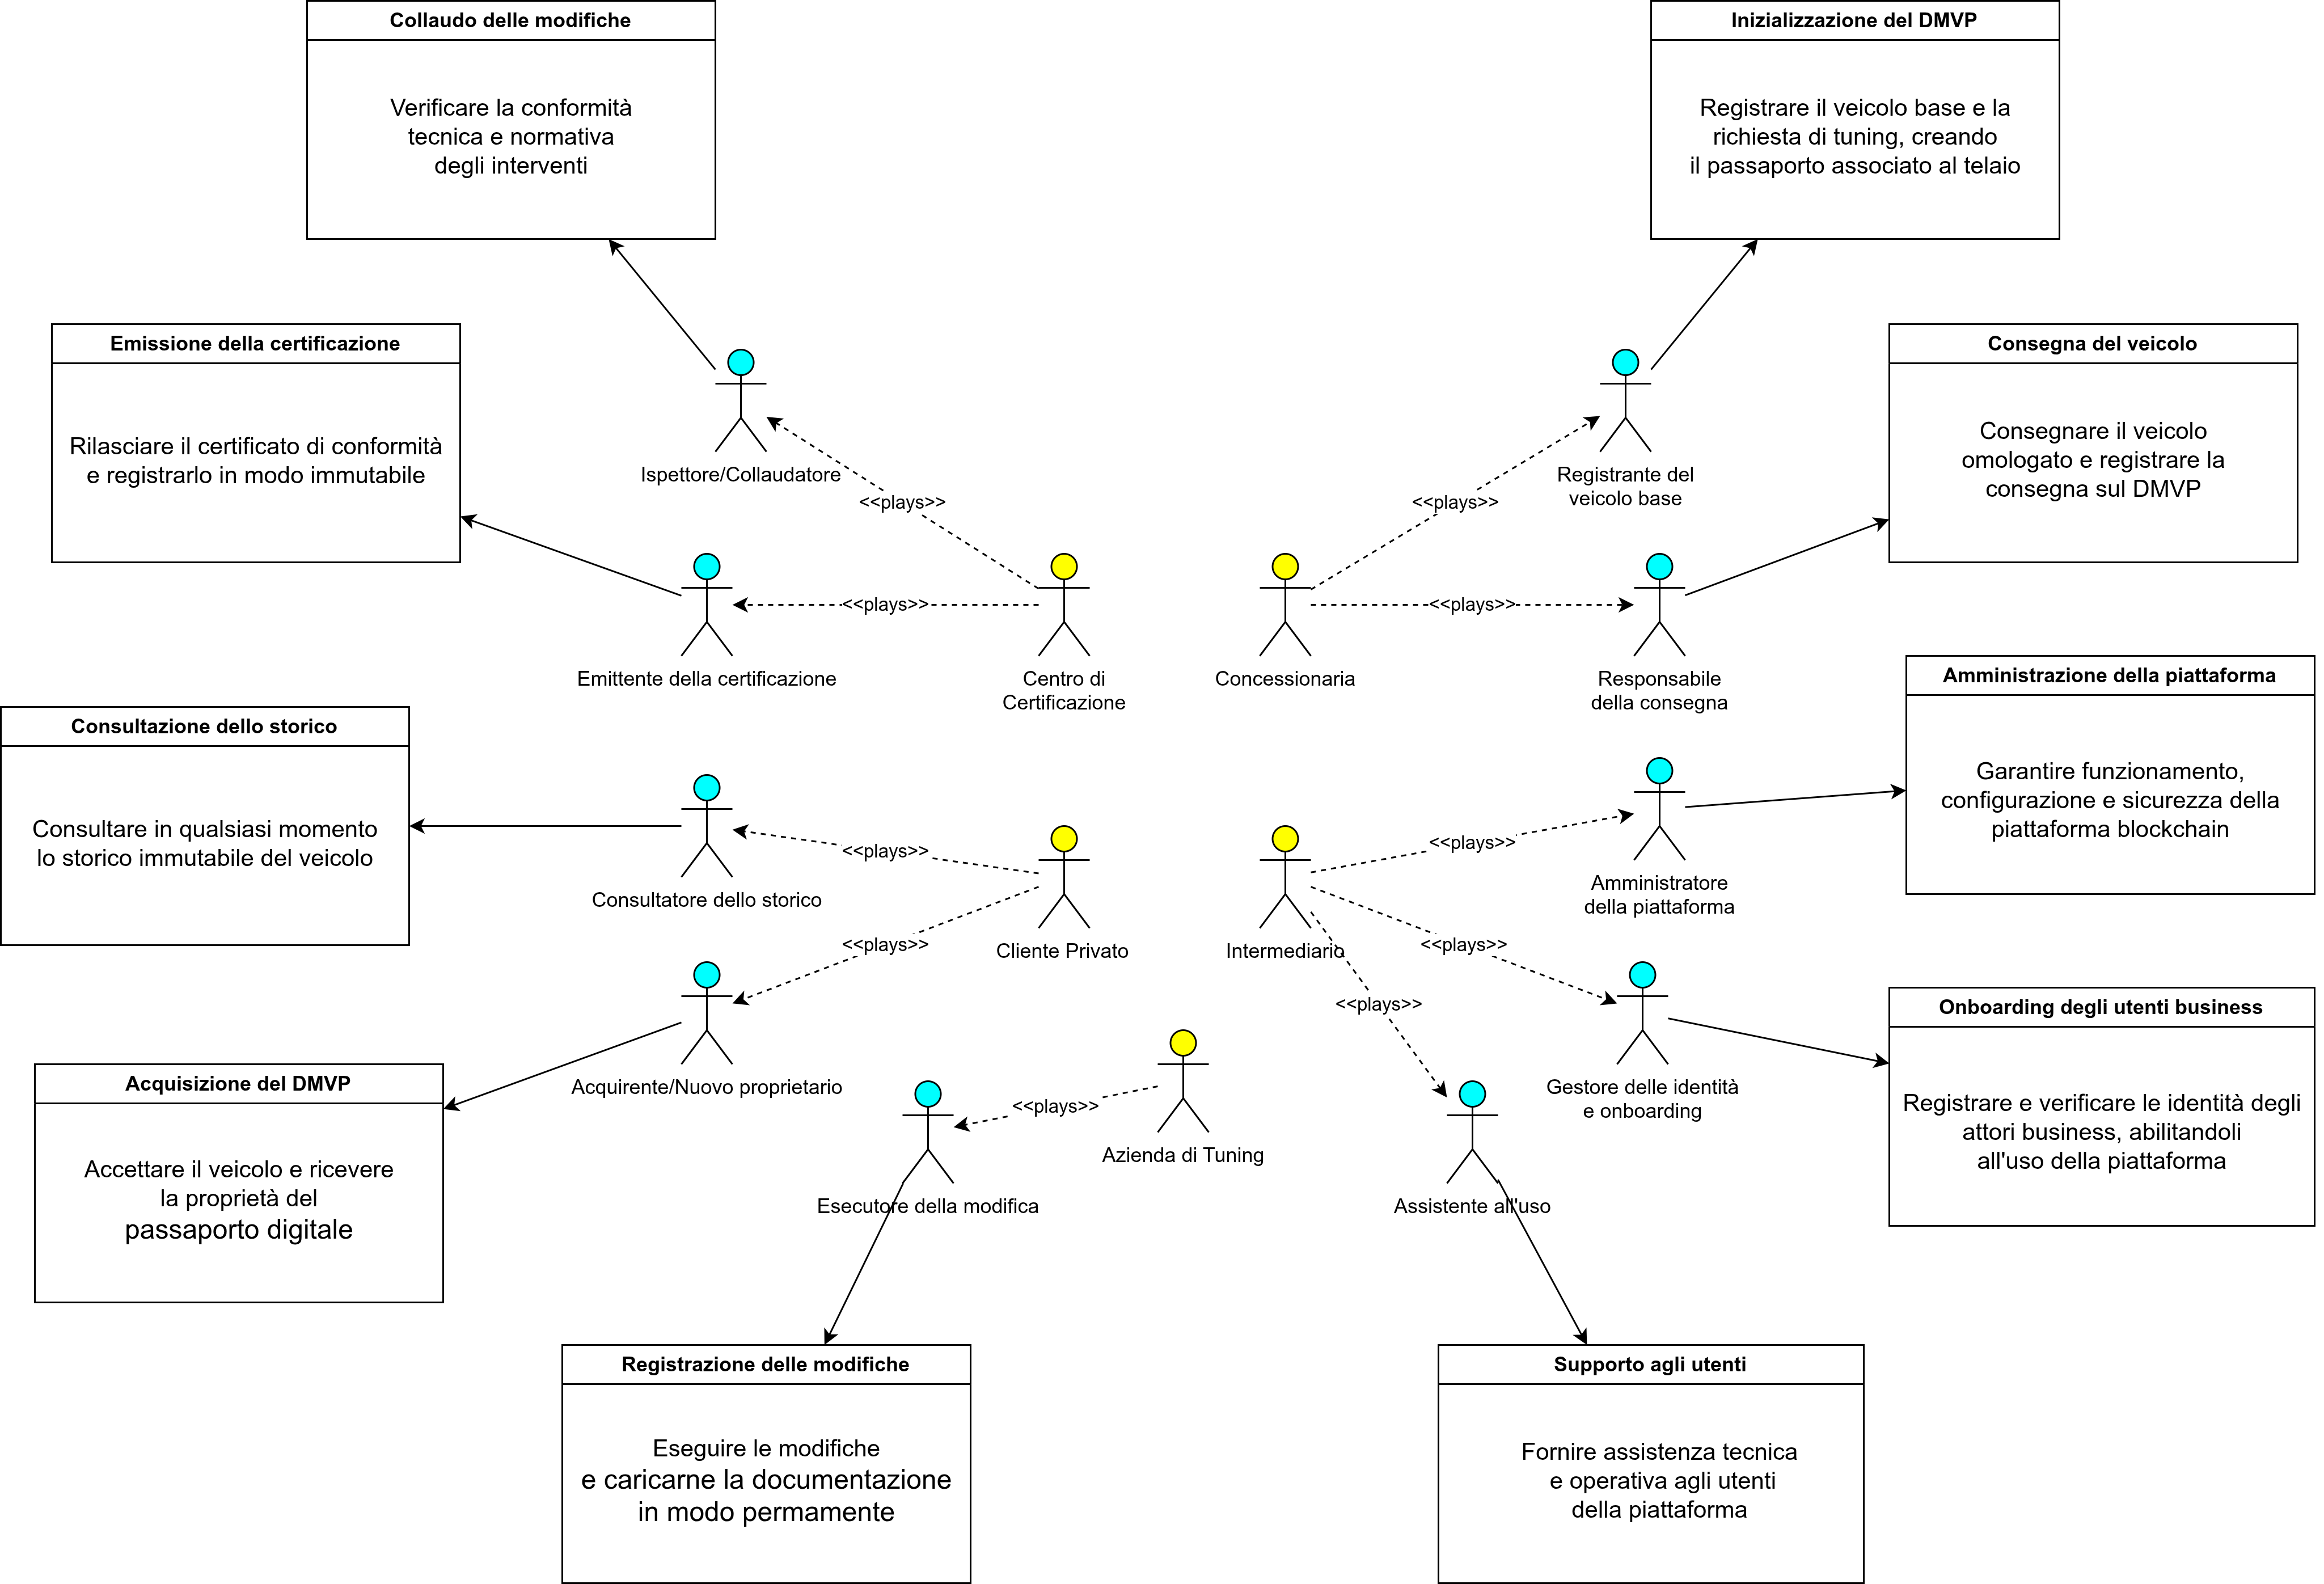
\includegraphics[width=\textwidth]{imgs/scenario/goal_diagram.png}
    \caption{Goal Diagram}
    \label{fig:goal-diagram}
\end{figure}

Se il Goal Diagram serve a isolare e definire i traguardi singoli di ogni ruolo, il \textbf{Goal Dependency Diagram} (Figura~\ref{fig:goal-dependency}) sposta l'attenzione sulla rete di relazioni e influenze che intercorrono tra di essi. L'obiettivo di questa rappresentazione è rendere esplicito come il raggiungimento di un fine possa agevolare (+) o, al contrario, ostacolare ($-$) le finalità degli altri ruoli coinvolti nel sistema.

\begin{figure}[H]
    \centering
    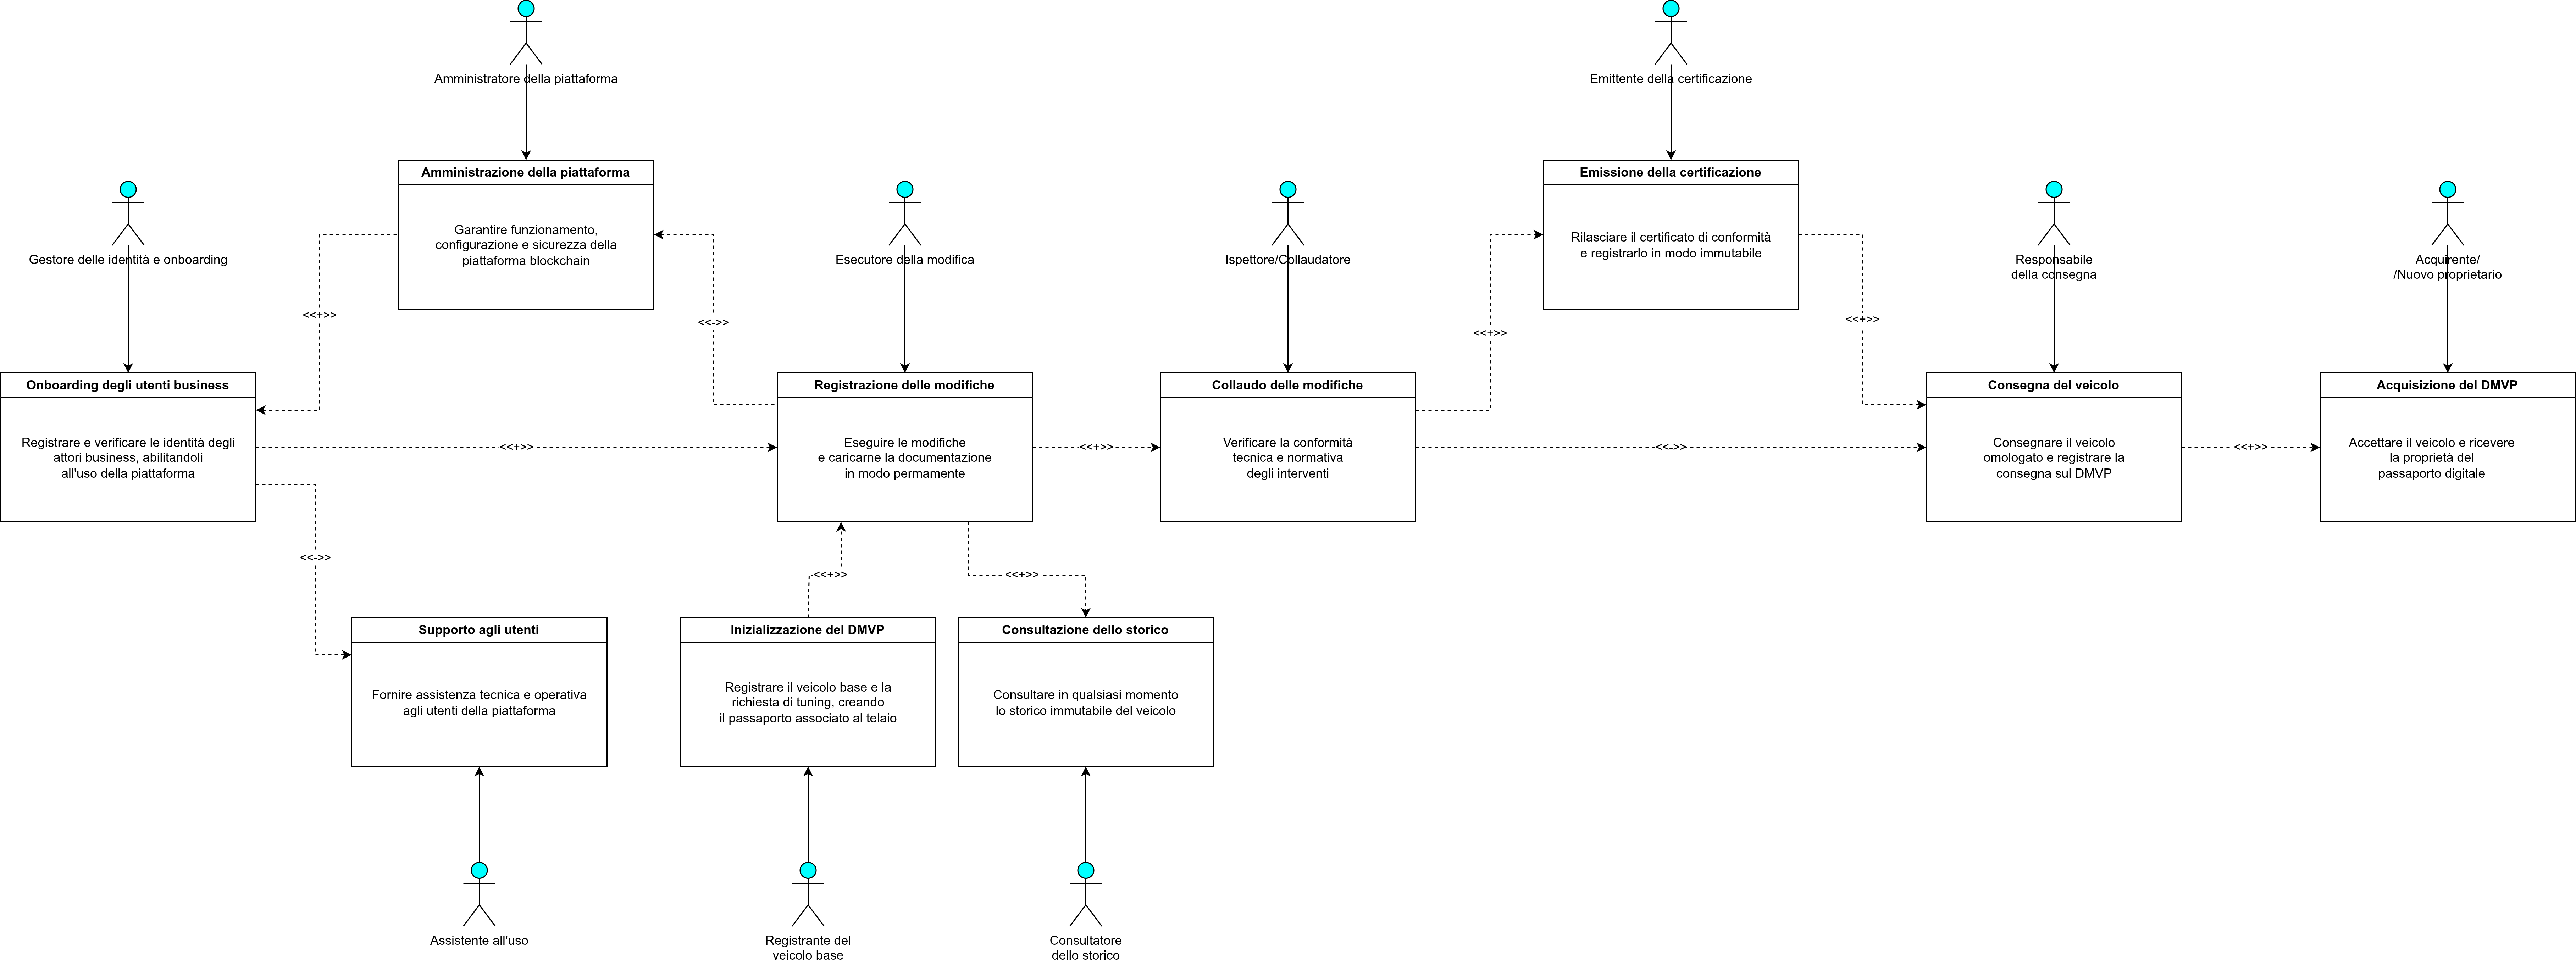
\includegraphics[width=\textwidth]{imgs/scenario/goal_dependency_diagram.png}
    \caption{Goal Dependency Diagram}
    \label{fig:goal-dependency}
\end{figure}

Vediamo nel dettaglio ogni dipendenza.

\subsection*{Contributes (+)}

\begin{itemize}
    \item \textbf{Amministrazione della piattaforma \quad$+$\quad Onboarding degli utenti business}\\
    Un'infrastruttura correttamente configurata e sicura costituisce il presupposto tecnico per poter abilitare nuovi attori: senza una rete permissioned funzionante e una Certification Authority operativa non sarebbe possibile emettere credenziali valide né ammettere organizzazioni al canale.

    \item \textbf{Onboarding degli utenti business \quad$+$\quad Registrazione delle modifiche}\\
    La verifica preventiva dell'identità degli attori garantisce che soltanto soggetti accreditati possano scrivere sul registro. Ne consegue che ogni lavorazione registrata è riconducibile in modo certo a un'azienda verificata, aumentando l'affidabilità del dato prodotto.

    \item \textbf{Inizializzazione del DMVP \quad$+$\quad Registrazione delle modifiche}\\
    L'esistenza del passaporto digitale associato al numero di telaio è la condizione necessaria affinché le modifiche possano esservi ancorate: senza l'istanza creata dalla Concessionaria, l'Azienda di Tuning non avrebbe alcun registro su cui operare.

    \item \textbf{Registrazione delle modifiche \quad$+$\quad Collaudo delle modifiche}\\
    Una documentazione tecnica completa, strutturata e immutabile consente al collaudatore di svolgere le verifiche in modo più rapido e oggettivo, evitando la ricostruzione manuale della storia degli interventi.

    \item \textbf{Collaudo delle modifiche \quad$+$\quad Emissione della certificazione}\\
    L'esito documentato delle verifiche tecniche e normative è il presupposto formale per il rilascio del certificato di conformità: senza collaudo non vi è alcuna base su cui fondare la certificazione.

    \item \textbf{Emissione della certificazione \quad$+$\quad Consegna del veicolo}\\
    La disponibilità del certificato registrato in modo immutabile abilita la Concessionaria ad avviare la procedura di consegna, potendo dimostrare la piena regolarità del veicolo modificato.

    \item \textbf{Consegna del veicolo \quad$+$\quad Acquisizione del DMVP}\\
    La consegna formale del veicolo omologato è ciò che innesca il trasferimento della proprietà del passaporto digitale all'account del Cliente Privato, completando il ciclo di tracciabilità.

    \item \textbf{Registrazione delle modifiche \quad$+$\quad Consultazione dello storico}\\
    Quanto più le lavorazioni vengono registrate in modo puntuale e dettagliato, tanto più lo storico consultabile dal Cliente Privato risulta completo e significativo ai fini della verifica di autenticità e della valorizzazione del veicolo.
\end{itemize}

\subsection*{Hinders ($-$)}

\begin{itemize}
    \item \textbf{Registrazione delle modifiche \quad$-$\quad Amministrazione della piattaforma}\\
    Il volume crescente di documentazione caricata e di ancoraggi sulla catena appesantisce la gestione dell'infrastruttura, incrementando i requisiti di storage, il carico sui nodi e l'onere di monitoraggio a carico dell'Intermediario.

    \item \textbf{Onboarding degli utenti business \quad$-$\quad Supporto agli utenti}\\
    L'ampliamento della base di attori abilitati genera un corrispondente aumento delle richieste di assistenza e di formazione, rendendo più difficile mantenere gli stessi livelli di servizio a parità di risorse dedicate al supporto.

    \item \textbf{Collaudo delle modifiche \quad$-$\quad Consegna del veicolo}\\
    Il rigore delle verifiche tecniche e normative, pur necessario a garantire la conformità, allunga i tempi complessivi del processo e può ritardare la consegna del veicolo al cliente, soprattutto qualora il collaudo dia esito negativo e imponga interventi correttivi.
\end{itemize}

\section{Modello di Business dell'Idea Progettuale in Canvas}

\subsection{Schema del Modello di Business dell'Idea Progettuale}

La Figura~\ref{fig:canvas} illustra il modello di business dell'idea progettuale, realizzato con il formalismo Canvas. Il modello è costruito attorno all'individuazione dell'\textbf{Intermediario} quale cliente primario della piattaforma e organizza il valore offerto per segmento, in modo che a ciascuno stakeholder corrisponda la proposta di valore che ne motiva l'adesione.

\begin{figure}[H]
    \centering
    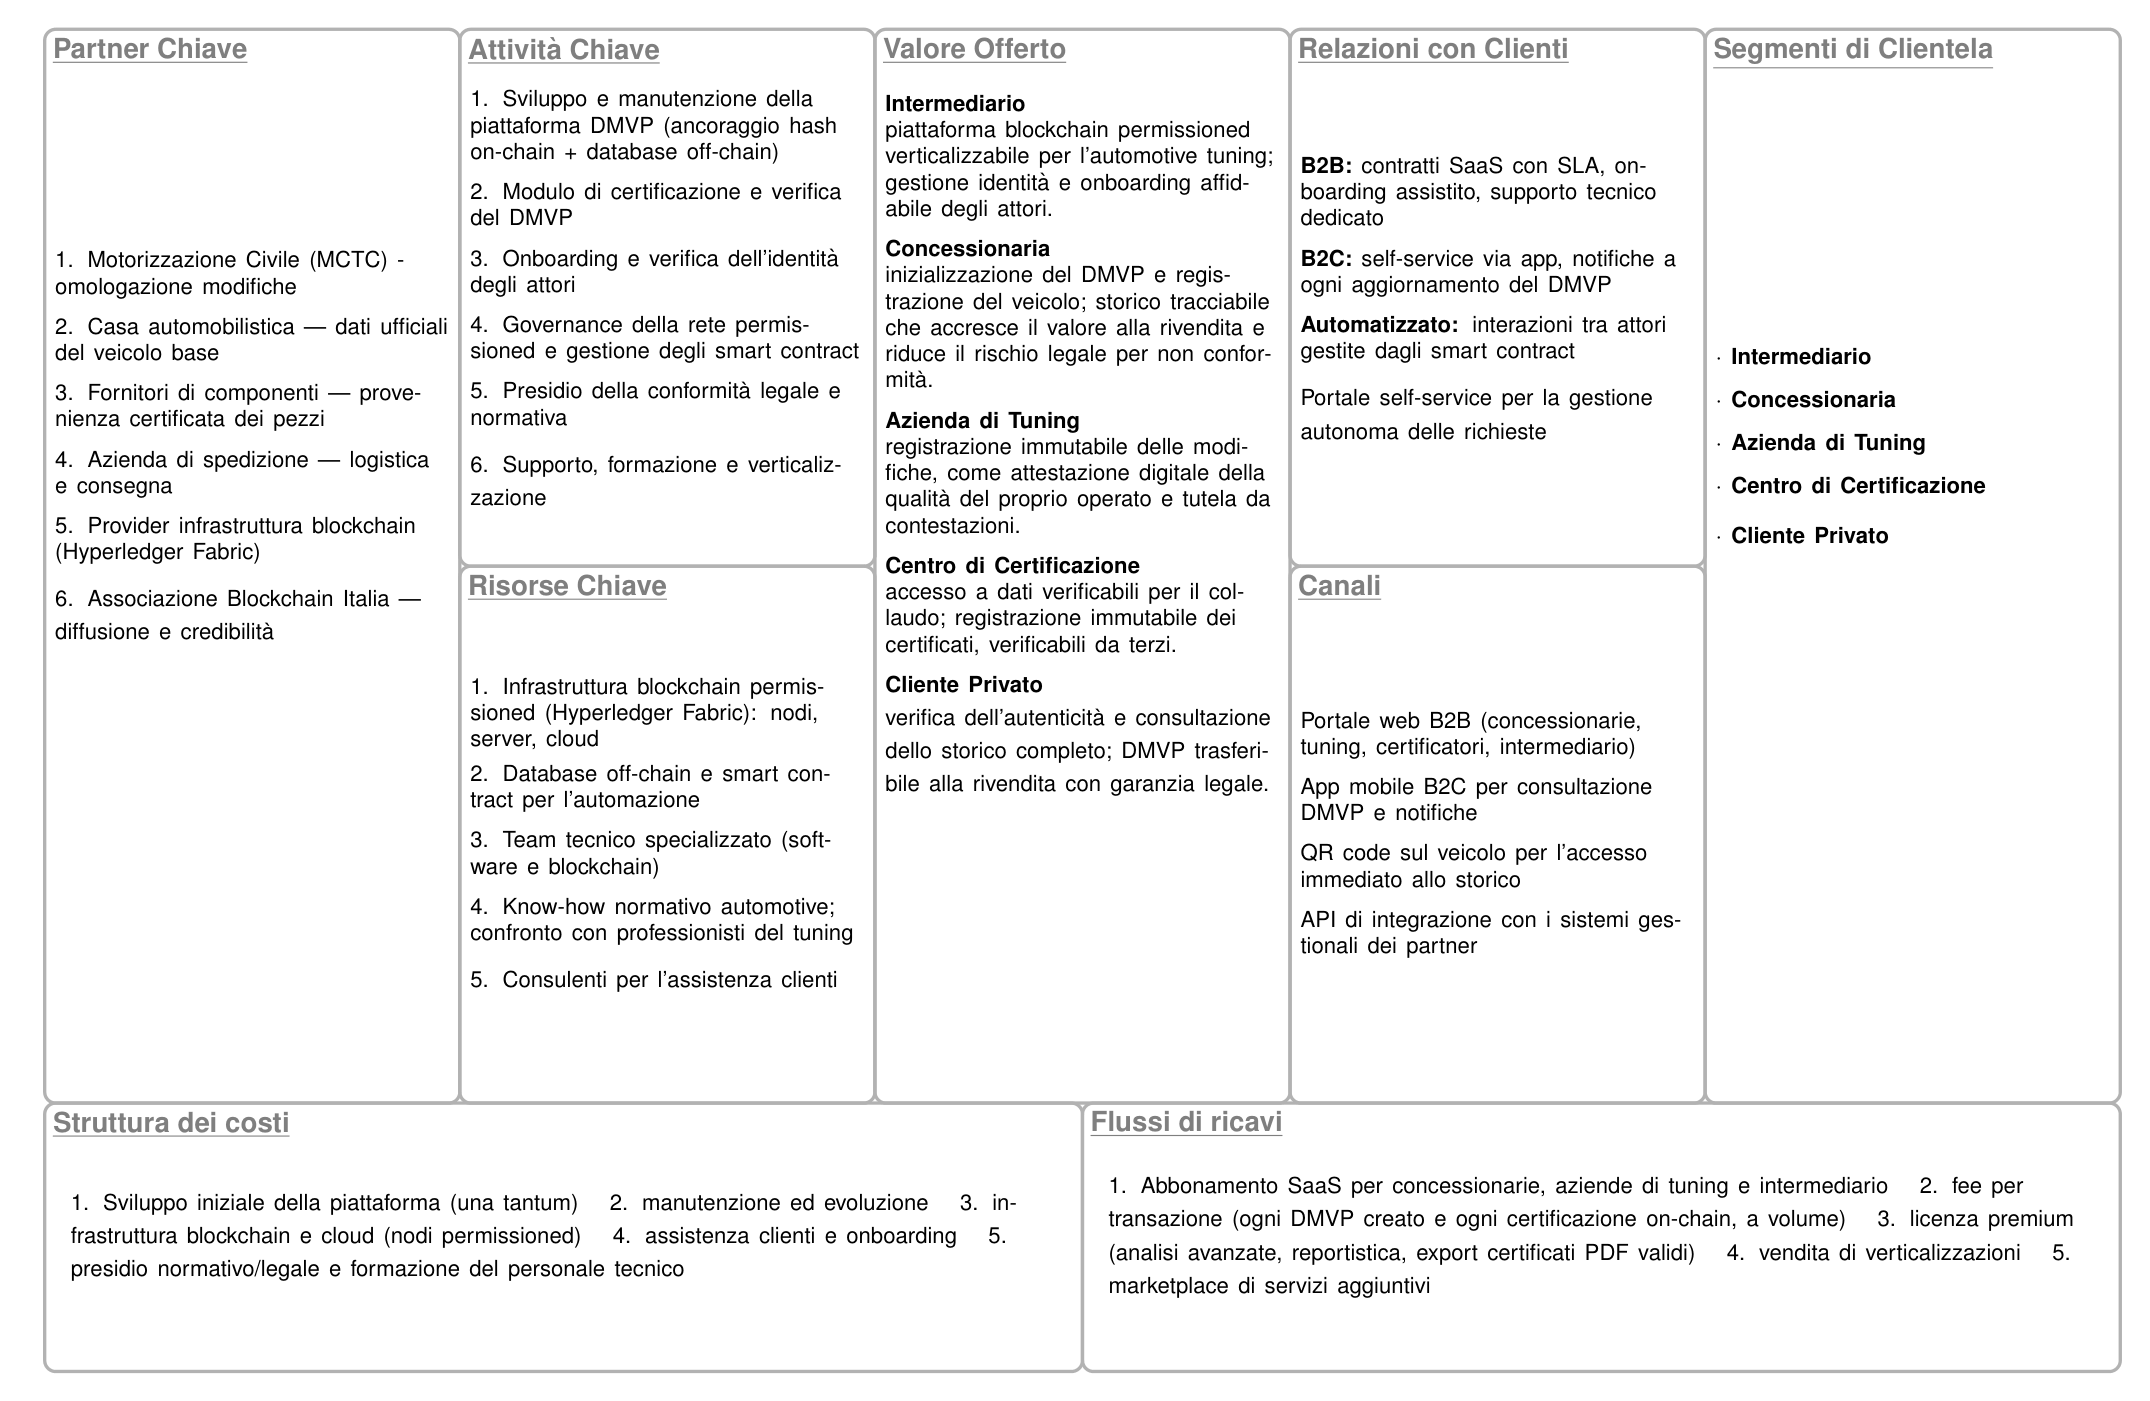
\includegraphics[width=\textwidth]{imgs/scenario/business_model_canvas.png}
    \caption{Modello di Business in Canvas}
    \label{fig:canvas}
\end{figure}

\subsection{Descrizione in dettaglio del Modello di Business}

\subsubsection*{Partner Chiave}

\begin{itemize}
    \item \textbf{Motorizzazione Civile (MCTC)}: ente competente per l'omologazione delle modifiche apportate ai veicoli. Rappresenta il partner istituzionale di riferimento, la cui collaborazione è determinante per il riconoscimento formale del DMVP.
    \item \textbf{Casa automobilistica}: fornisce i dati ufficiali del veicolo base, necessari all'inizializzazione del passaporto digitale.
    \item \textbf{Fornitori di componenti}: attestano la provenienza certificata dei pezzi installati, consentendo di estendere la tracciabilità anche a monte della lavorazione.
    \item \textbf{Azienda di spedizione}: gestisce la logistica e la consegna del veicolo, fase che il DMVP registra come passaggio di responsabilità.
    \item \textbf{Provider dell'infrastruttura blockchain}: fornisce la tecnologia su cui poggia la rete permissioned.
    \item \textbf{Associazione Blockchain Italia}: organizzazione no-profit attiva nella promozione delle tecnologie DLT, partner strategico per il posizionamento istituzionale della soluzione e la sensibilizzazione degli stakeholder.
\end{itemize}

\subsubsection*{Attività Chiave}

Le attività chiave comprendono lo sviluppo e la manutenzione della piattaforma DMVP, nella duplice componente di ancoraggio degli hash on-chain e di gestione del database off-chain; lo sviluppo del modulo di certificazione e verifica del passaporto; l'onboarding e la verifica dell'identità degli attori; la governance della rete permissioned e la gestione degli smart contract; il presidio della conformità legale e normativa, particolarmente critico in un settore regolamentato come quello dell'omologazione veicolare; e infine le attività di supporto, formazione e verticalizzazione della piattaforma.

\subsubsection*{Risorse Chiave}

Le risorse chiave sono costituite dall'infrastruttura blockchain permissioned, comprensiva di nodi, server e servizi cloud; dal database off-chain e dagli smart contract per l'automazione dei processi; dal team tecnico specializzato in sviluppo software e tecnologie a registro distribuito; dal know-how normativo in ambito automotive, alimentato dal confronto con i professionisti del settore; e dai consulenti a supporto dell'assistenza clienti.

\subsubsection*{Valore Offerto}

Il valore offerto è articolato per segmento, in modo che ciascuna proposta risulti direttamente riconducibile ai casi d'uso descritti nel capitolo seguente:

\begin{itemize}
    \item \textbf{Intermediario}: piattaforma blockchain permissioned verticalizzabile per la filiera dell'automotive tuning, con gestione affidabile delle identità e dell'onboarding degli attori.
    \item \textbf{Concessionaria}: inizializzazione del DMVP e registrazione del veicolo; storico tracciabile che ne accresce il valore alla rivendita e riduce il rischio legale per non conformità.
    \item \textbf{Azienda di Tuning}: registrazione immutabile delle modifiche eseguite, quale attestazione digitale della qualità del proprio operato e tutela da contestazioni.
    \item \textbf{Centro di Certificazione}: accesso a dati verificabili per il collaudo e registrazione immutabile dei certificati emessi, controllabili da terzi.
    \item \textbf{Cliente Privato}: verifica dell'autenticità e consultazione dello storico completo del veicolo; passaporto digitale trasferibile alla rivendita.
\end{itemize}

\subsubsection*{Relazioni con i Clienti}

La relazione con i clienti si articola su tre modalità. Sul versante \textbf{B2B} si adottano contratti SaaS con livelli di servizio definiti, onboarding assistito e supporto tecnico dedicato, coerentemente con la natura tecnica dell'infrastruttura. Sul versante \textbf{B2C} la relazione è di tipo self-service attraverso l'applicazione mobile, con notifiche automatiche a ogni aggiornamento del DMVP. Una componente \textbf{automatizzata} è infine garantita dagli smart contract, che gestiscono le interazioni tra attori senza necessità di coordinamento manuale. A queste si affianca un portale self-service per la gestione autonoma delle richieste.

\subsubsection*{Canali}

La distribuzione avviene attraverso un portale web B2B destinato a concessionarie, aziende di tuning, centri di certificazione e intermediario; un'applicazione mobile B2C per la consultazione del DMVP e la ricezione delle notifiche; un QR code applicato al veicolo, che consente l'accesso immediato allo storico anche a un potenziale acquirente; e infine API di integrazione con i sistemi gestionali dei partner.

\subsubsection*{Segmenti di Clientela}

I segmenti di clientela coincidono con gli stakeholder dello scenario specifico: Intermediario, Concessionaria, Azienda di Tuning, Centro di Certificazione e Cliente Privato. Tra questi, l'\textbf{Intermediario} riveste il ruolo di cliente primario, in quanto soggetto che acquisisce la piattaforma e ne cura la verticalizzazione presso gli altri attori della filiera.

\subsubsection*{Struttura dei Costi}

La struttura dei costi comprende lo sviluppo iniziale della piattaforma, sostenuto una tantum; la manutenzione e l'evoluzione del sistema; l'infrastruttura blockchain e cloud, con particolare riferimento all'esercizio dei nodi permissioned; l'assistenza clienti e l'onboarding; e infine il presidio normativo e legale, unitamente alla formazione del personale tecnico. L'analisi economica dettagliata di tali voci è sviluppata nel Business Plan (Capitolo~7).

\subsubsection*{Flussi di Ricavi}

I flussi di ricavo previsti sono di natura prevalentemente B2B e comprendono l'abbonamento SaaS per concessionarie, aziende di tuning e intermediario; una fee per transazione proporzionale al volume di DMVP creati e di certificazioni registrate on-chain; una licenza premium per analisi avanzate, reportistica ed esportazione di certificati in formato legalmente valido; la vendita di verticalizzazioni della piattaforma; e un marketplace di servizi aggiuntivi.